%%% Template originaly created by Karol Kozioł (mail@karol-koziol.net) and modified for ShareLaTeX use

\documentclass[a4paper,11pt]{article}

\usepackage[T1]{fontenc}
\usepackage[utf8]{inputenc}
\usepackage{graphicx}
\usepackage{subcaption}
\usepackage{xcolor}
\usepackage{stmaryrd}

% \renewcommand\familydefault{\sfdefault}
% \usepackage{tgheros}
% \usepackage[defaultmono]{droidmono}
\usepackage{mathrsfs}

\usepackage{amsmath,amssymb,amsthm,textcomp}
\usepackage{enumerate}
\usepackage{multicol}
\usepackage{tikz}
\usepackage{hyperref}

\usepackage{geometry}
\geometry{left=25mm,right=25mm,%
bindingoffset=0mm, top=20mm,bottom=20mm}

\usepackage[table]{xcolor} % Para colorear tablas
\usepackage{colortbl}      % Necesario para \cellcolor
\usepackage{array}         % Para centrar texto en columnas

\setlength{\parskip}{1em}
%\linespread{1.3}

\newcommand{\linia}{\rule{\linewidth}{0.5pt}}

% % custom theorems if needed
% \newtheoremstyle{mytheor}
%     {1ex}{1ex}{\normalfont}{0pt}{\scshape}{.}{1ex}
%     {{\thmname{#1 }}{\thmnumber{#2}}{\thmnote{ (#3)}}}
%
% \theoremstyle{mytheor}
% \newtheorem{defi}{Definition}

% my own titles
\makeatletter
\renewcommand{\maketitle}{
\begin{center}
\vspace{2ex}
{\Large \textsc{\@title}}
\vspace{1ex}
\\
\linia\\
\@author \hfill \@date
\vspace{4ex}
\end{center}
}
\makeatother
%%%

% custom footers and headers
\usepackage{fancyhdr}
\pagestyle{fancy}
\lhead{}
\chead{}
\rhead{}
%\lfoot{Lógica Proposicional}
\cfoot{}
%\rfoot{página \thepage}
\renewcommand{\headrulewidth}{0pt}
\renewcommand{\footrulewidth}{0pt}
%

% code listing settings
\usepackage{listings}
\lstset{
    language=Python,
    basicstyle=\ttfamily\small,
    aboveskip={1.0\baselineskip},
    belowskip={1.0\baselineskip},
    columns=fixed,
    extendedchars=true,
    breaklines=true,
    tabsize=4,
    prebreak=\raisebox{0ex}[0ex][0ex]{\ensuremath{\hookleftarrow}},
    frame=lines,
    xleftmargin=2em,
    framexleftmargin=2em,
    showtabs=false,
    showspaces=false,
    showstringspaces=false,
    keywordstyle=\color[rgb]{0.627,0.126,0.941},
    commentstyle=\color[rgb]{0.133,0.545,0.133},
    stringstyle=\color[rgb]{01,0,0},
    numbers=left,
    numberstyle=\small,
    stepnumber=1,
    numbersep=5pt,
    captionpos=t,
    escapeinside={\%*}{*)}
}

%% SET THEORY %%

\usepackage{mathtools}
\usepackage{xparse}
\DeclarePairedDelimiterX\set[2]{\{}{\}}{\,#1 \;\delimsize\vert\; #2\,}

\newcommand{\eqdef}{\stackrel{\text{def}}{=}}

%% local labels in equations %%

\usepackage{xargs}

\makeatletter
  \newcommandx{\Label}[1][1={\arabic{equation}}]%
    {\refstepcounter{equation}(\theequation)~\ltx@label{{#1}} &&}
\makeatother

%% Proof trees %%

\usepackage{fitch}

\usepackage{etoolbox}
\let\bbordermatrix\bordermatrix
\patchcmd{\bbordermatrix}{8.75}{4.75}{}{}
\patchcmd{\bbordermatrix}{\left(}{\left[}{}{}
\patchcmd{\bbordermatrix}{\right)}{\right]}{}{}

%% circled question mark %%

\usepackage{tikz}
\newcommand*\circled[1]{\tikz[baseline=(char.base)]{
            \node[shape=circle,draw,inner sep=.7pt] (char) {\footnotesize #1};}}
\newcommand{\result}{\circled{?}}

%% Venn Diagrams %%

\usepackage{venndiagram}

%% LOGICAL SYMBOLS %%

\newcommand{\liff}{\leftrightarrow}
\DeclarePairedDelimiterX\FORALL[3]{(}{)}{\,\forall #1 : #2 : #3 \,}
\DeclarePairedDelimiterX\EXISTS[3]{(}{)}{\,\exists #1 : #2 : #3 \,}
\DeclarePairedDelimiterX\eval[1]{\llbracket}{\rrbracket}{#1}
\newcommand{\sem}[1]{\eval{#1}^{\model}}
\newcommand{\semv}[2]{\eval{#2}^{\model,#1}}
\newcommand{\model}{\mathfrak{M}}
\newcommand{\interpretation}{\mathscr{I}}
\DeclareMathOperator{\dom}{dom}
\DeclareMathOperator{\fun}{fun}
\DeclareMathOperator{\rel}{rel}

\DeclareRobustCommand{\svdots}{% s for `scaling'
  \vcenter{%
    \offinterlineskip
    \vspace{5pt}
    \hbox{.}
    \vskip0.25\normalbaselineskip
    \hbox{.}
    \vskip0.25\normalbaselineskip
    \hbox{.}%
  }%
}

%% COMPLETE BOX %%
\def\fillbox{\quad[\qquad]\quad}

%% NO INDENT %%

\setlength{\parindent}{0pt}

%%%% LOCALDEFS %%%%

\newcommand{\ambassador}{\mathsf{ambassador}_1}
\newcommand{\person}{\mathsf{person}_1}
\newcommand{\country}{\mathsf{country}_1}
\newcommand{\sentto}{\mathsf{sentto}_2}
\newcommand{\knight}{\mathsf{knight}_1}
\newcommand{\knave}{\mathsf{knave}_1}
\newcommand{\alice}{\mathsf{alice}}
\newcommand{\bob}{\mathsf{bob}}
\newcommand{\tom}{\mathsf{tom}}
\newcommand{\carl}{\mathsf{carl}}

\newcommand{\assig}{\cellcolor{gray!30}1}
\newcommand{\conf}{\cellcolor{yellow!40}1}
\newcommand{\void}{\cellcolor{white}0}

%%%----------%%%----------%%%----------%%%----------%%%

\begin{document}

\title{Coloreo de grafos}

\author{Lautaro Luna}

\date{}

\maketitle

\vspace*{-1cm}

\tableofcontents  % <-- Esto genera el índice
\newpage

\section{Coloreo de grafos}
Considerando el siguiente grafo:

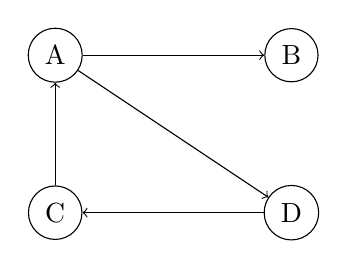
\begin{tikzpicture}
    \centering
    \node[draw, circle] (A) at (0,2) {A};
    \node[draw, circle] (B) at (3,2) {B};
    \node[draw, circle] (C) at (0,0) {C};
    \node[draw, circle] (D) at (3,0) {D};

    \draw[->] (A) -- (B);  % Flecha de A a B
    \draw[->] (A) -- (D);
    \draw[->] (C) -- (A);
    \draw[->] (D) -- (C);
\end{tikzpicture}

\subsection{Reestricciones del problema}

\subsubsection{Las aristas son sólo entre nodos}
\begin{equation}
    (\forall s, t\;::\; edge_2(s, t) \rightarrow node_1(s) \land node_1(t))
\end{equation}

\subsubsection{El coloreo es entre nodo y color}
\begin{equation}
    (\forall n :: (\forall c :: coloring_2(n, c) \rightarrow node_1(n) \land color_1(c) ) )
\end{equation}

\subsubsection{Todo nodo tiene un único color}
\begin{equation}
    (\forall n, c, c' :: (coloring_2(n, c) \land coloring_2(n, c')) \rightarrow eq_2(c, c'))
\end{equation}

\subsubsection{No hay nodos adyacentes con el mismo color}
\begin{equation}
    \neg (\exists s, t, c :: edge_2(s, t) \land coloring_2(s, c) \land coloring_2(t, c))
\end{equation}

\subsubsection{Los nodos no son colores y los colores no son nodos}
\begin{equation}
    (\forall x :: node_1(x) \lor color_1(x)) \land \neg (\exists x :: node_1(x) \land color_1(x))
\end{equation}

\subsubsection{Tengo sólo 3 colores}
\begin{multline}
    color_1(C1) \land color_1(C2) \land color_1(C3) \\
    \land (C1 \not= C2) \land (C2 \not= C3) \land (C1 \not= C3) \\
    (\forall c :: color_1(c) \rightarrow c = C1 \lor c = C2 \lor c = C3) \\
\end{multline}

\newpage

\begin{center}
    \textbf{$node_1$} \\[4pt]
    \renewcommand{\arraystretch}{1.5} % <-- Aumenta el espacio entre filas
    \begin{tabular}{@{}c@{\hskip 1em}>{\columncolor{blue!80!white}\color{white}}c@{}}
        0 & 1 \\
        1 & 1 \\
        2 & 1 \\
        3 & 1 \\
        4 & 0 \\
        5 & 0 \\
        6 & 0 \\
    \end{tabular}
\end{center}

\newpage

\section{Club de lectura}

Se analiza un modelo lógico para representar la estructura de un club de lectura, utilizando predicados que distinguen entre miembros, novelas de misterio y novelas de ciencia ficción, así como la relación de gusto entre ellos.

\subsection{Modelo que no debería ser permitido}

\begin{center}
    \begin{minipage}{0.23\textwidth}
        \centering
        \textbf{$member_1$ ($\phi$) } \\[4pt]
        \begin{tabular}{@{}c@{\hskip 1em}>{\columncolor{blue!80!white}\color{white}}c@{}}
            0 & 1 \\
            1 & 1 \\
            2 & 0 \\
            3 & 0 \\
        \end{tabular}
    \end{minipage}
    \begin{minipage}{0.23\textwidth}
        \centering
        \textbf{$mysteryNovel_1$ ($\psi$)} \\[4pt]
        \begin{tabular}{@{}c@{\hskip 1em}>{\columncolor{blue!80!white}\color{white}}c@{}}
            0 & 0 \\
            1 & 1 \\
            2 & 1 \\
            3 & 0 \\
        \end{tabular}
    \end{minipage}
    \begin{minipage}{0.23\textwidth}
        \centering
        \textbf{$scifiNovel_1$ ($\omega$)} \\[4pt]
        \begin{tabular}{@{}c@{\hskip 1em}>{\columncolor{blue!80!white}\color{white}}c@{}}
            0 & 0 \\
            1 & 0 \\
            2 & 0 \\
            3 & 1 \\
        \end{tabular}
    \end{minipage}
    \begin{minipage}{0.23\textwidth}
        \centering
        \textbf{$likes_2$} \\[4pt]
        \begin{tabular}{c@{\hskip 1em}*{4}{>{\columncolor{blue!80!white}\color{white}}c}}
            % Encabezado con fondo blanco y texto negro
            \rowcolor{white}
            \multicolumn{1}{>{\columncolor{white}\color{black}}c}{}  &
            \multicolumn{1}{>{\columncolor{white}\color{black}}c}{0} &
            \multicolumn{1}{>{\columncolor{white}\color{black}}c}{1} &
            \multicolumn{1}{>{\columncolor{white}\color{black}}c}{2} &
            \multicolumn{1}{>{\columncolor{white}\color{black}}c}{3}                 \\
            % Celdas de la matriz
            0                                                        & 0 & 0 & 0 & 0 \\
            1                                                        & 0 & 0 & 0 & 0 \\
            2                                                        & 0 & 0 & 0 & 0 \\
            3                                                        & 0 & 0 & 0 & 0 \\
        \end{tabular}
    \end{minipage}
\end{center}
\begin{center}
    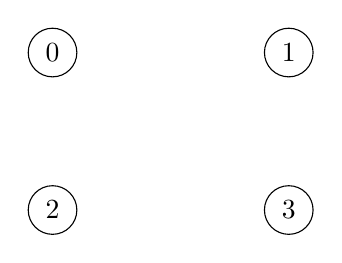
\begin{tikzpicture}
        \centering
        \node[draw, circle] (0) at (0,2) {0};
        \node[draw, circle] (1) at (3,2) {1};
        \node[draw, circle] (2) at (0,0) {2};
        \node[draw, circle] (3) at (3,0) {3};

    \end{tikzpicture}
\end{center}

\subsection{Valuación}
\begin{center}
    $\eval{\; (\forall x (\text{isMember}(x) \rightarrow \neg (\text{isMysteryNovel}(x) \lor \text{isSciFiNovel}(x))) \; \land
            (\forall x ((\text{isMysteryNovel}(x) \lor \text{isSciFiNovel}(x)) \rightarrow \neg \text{isMember}(x))) \;} = 0$
\end{center}
\textbf{Para todo x, si x es un miembro, entonces x no es una novela de misterio o una novela de ciencia ficción. Y para todo x, si x es una novela de misterio o una novela de ciencia ficción, entonces x no es un miembro.}
En otras palabras, esta fórmula indica que un miembro no puede ser ningún tipo de novela, y si es alguno de los tipos de novelas, no es un miembro.

\subsection{Justificación en modelo no permitido}

$
    \begin{nd}
        \hypo{}{\eval{{(\forall x (\phi(x) \rightarrow \neg (\psi(x) \lor \omega(x))) \land (\forall x ((\psi(x) \lor \omega(x)) \rightarrow \neg \phi(x)))}}}
        \have{}{min (\eval{\phi}, \eval{\psi})}

        \open
        \hypo{}{\eval{(\forall x (\phi(x) \rightarrow \neg (\psi(x) \lor \omega(x)))} }
        \have{}{min}

        \open
        \hypo{}{\eval{\phi(x) \rightarrow \neg (\psi(x) \lor \omega(x)}  \textbf{ cuando x = 1} }
        \have{}{max(1-\eval{\phi(x)} ,\eval{\neg (\psi(x) \lor \omega(x)})}
        \open
        \hypo{}{\eval{\phi(x)}}
        \have{}{1}
        \close
        \open
        \hypo{}{\eval{\neg (\psi(x) \lor \omega(x))} }
        \have{}{1-\eval{(\psi(x) \lor \omega(x))} }

        \open
        \hypo{}{\eval{\psi(x) \lor \omega(x)} }
        \have{}{max(\eval{(\psi(x)}, \eval{\omega(x)} }
        \open
        \hypo{}{\eval{\psi(x)}}
        \have{}{1}

        \close
        \open
        \hypo{}{\eval{\omega(x)} }
        \have{}{0}

        \close
        \have{}{1}
        \close
        \have{}{0}
        \close



        \have{}{max(1- 1, 0)}
        \have{}{max(0, 0)}
        \have{}{0}
        \close

        \have{}{0}
        \close

        \have{}{\eval{\phi}}
        \have{}{0}

    \end{nd}
$

En este caso, tomamos x = 1. La fórmula que propusimos da falsa; con x = 1, x es en este modelo a la vez, un miembro y una novela de misterio, pero establecimos formalmente que este caso no puede darse.


\newpage

\subsection{Modelo bueno}

\begin{center}
    \begin{minipage}{0.23\textwidth}
        \centering
        \textbf{$member_1$ ($\phi$) } \\[4pt]
        \begin{tabular}{@{}c@{\hskip 1em}>{\columncolor{blue!80!white}\color{white}}c@{}}
            0 & 1 \\
            1 & 1 \\
            2 & 0 \\
            3 & 0 \\
        \end{tabular}
    \end{minipage}
    \begin{minipage}{0.23\textwidth}
        \centering
        \textbf{$mysteryNovel_1$ ($\psi$)} \\[4pt]
        \begin{tabular}{@{}c@{\hskip 1em}>{\columncolor{blue!80!white}\color{white}}c@{}}
            0 & 0 \\
            1 & 0 \\
            2 & 1 \\
            3 & 0 \\
        \end{tabular}
    \end{minipage}
    \begin{minipage}{0.23\textwidth}
        \centering
        \textbf{$scifiNovel_1$ ($\omega$)} \\[4pt]
        \begin{tabular}{@{}c@{\hskip 1em}>{\columncolor{blue!80!white}\color{white}}c@{}}
            0 & 0 \\
            1 & 0 \\
            2 & 0 \\
            3 & 1 \\
        \end{tabular}
    \end{minipage}
    \begin{minipage}{0.23\textwidth}
        \centering
        \textbf{$likes_2$} \\[4pt]
        \begin{tabular}{c@{\hskip 1em}*{4}{>{\columncolor{blue!80!white}\color{white}}c}}
            % Encabezado con fondo blanco y texto negro
            \rowcolor{white}
            \multicolumn{1}{>{\columncolor{white}\color{black}}c}{}  &
            \multicolumn{1}{>{\columncolor{white}\color{black}}c}{0} &
            \multicolumn{1}{>{\columncolor{white}\color{black}}c}{1} &
            \multicolumn{1}{>{\columncolor{white}\color{black}}c}{2} &
            \multicolumn{1}{>{\columncolor{white}\color{black}}c}{3}                 \\
            % Celdas de la matriz
            0                                                        & 0 & 0 & 1 & 1 \\
            1                                                        & 0 & 0 & 0 & 0 \\
            2                                                        & 0 & 0 & 0 & 0 \\
            3                                                        & 0 & 0 & 0 & 0 \\
        \end{tabular}
    \end{minipage}
\end{center}

\begin{center}
    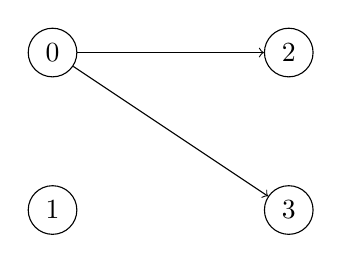
\begin{tikzpicture}
        \centering
        \node[draw, circle] (0) at (0,2) {0};
        \node[draw, circle] (1) at (0,0) {1};
        \node[draw, circle] (2) at (3,2) {2};
        \node[draw, circle] (3) at (3,0) {3};

        \draw[->] (0) -- (2);  % Flecha de A a B
        \draw[->] (0) -- (3);
    \end{tikzpicture}
\end{center}

\subsubsection{Evitar reflexión}
$(\forall x :: \neg likes_2(x, x))$

\subsubsection{A ningún miembro le puede gustar otro miembro}
$(\forall P1, P2 :: member_1(P1) \land member_1(P2) \land P1 \not= P2 \rightarrow \neg likes_2(P1, P2))$

\subsubsection{A ninguna novela le puede gustar otra novela}
$(\forall x, y :: (mysteryNovel_1(x) \lor scifiNovel_1(x)) \land (mysteryNovel_1(y) \lor scifiNovel_1(y)) \\ \rightarrow \neg likes_2(x, y))$

\subsubsection{A ninguna novela le puede gustar un miembro}
$(\forall x, p :: (mysteryNovel_1(x) \lor scifiNovel_1(x)) \land member_1(p) \rightarrow \neg likes_2(x, p))$

\subsubsection{Existe un miembro que le gusta una de cada tipo de novela}
$(\exists p, m, s :: member_1(p) \land mysteryNovel_1(m) \land scifiNovel_1(s) \land likes_2(p, m) \land likes_2(p, s))$

\newpage
Universo: 1, 2, 3
\begin{center}
    \begin{minipage}{0.23\textwidth}
        \centering
        \textbf{$G_2$} \\[4pt]
        \begin{tabular}{c@{\hskip 1em}*{4}{>{\columncolor{blue!80!white}\color{white}}c}}
            % Encabezado con fondo blanco y texto negro
            \rowcolor{white}
            \multicolumn{1}{>{\columncolor{white}\color{black}}c}{}  &
            \multicolumn{1}{>{\columncolor{white}\color{black}}c}{1} &
            \multicolumn{1}{>{\columncolor{white}\color{black}}c}{2} &
            \multicolumn{1}{>{\columncolor{white}\color{black}}c}{3}             \\
            1                                                        & 1 & 1 & 0 \\
            2                                                        & 1 & 1 & 1 \\
            3                                                        & 0 & 1 & 1 \\
        \end{tabular}
    \end{minipage}
\end{center}

\subsection{Lol}
Probar que: \\
$(\forall x, y :: G_2(x, y) \rightarrow G_2(x, y)$ \\
$
    \begin{nd}
        \hypo{}{\eval{(\forall x, y :: G_2(x, y) \rightarrow G_2(x, y)}}
        \have{}{min}

        \open
        \hypo{}{\eval{ G_2(x, y) \rightarrow G_2(x, y)}}
        \have{}{max(1 - \eval{G_2(x, y)}, \eval{G_2(y, x)}}

        \open
        \hypo{}{\eval{G_2(x, y)}}
        \have{}{?}
        \close

        \open
        \hypo{}{\eval{G_2(y, y)}}
        \have{}{?}
        \close

        \have{}{?}

        \close
        \have{}{?}

    \end{nd}
$

\newpage
\section{Problema de materias y franjas horarias}

Se presenta la siguiente situación problemática:

En la universidad, cursamos cinco materias: \textbf{Lógica}, \textbf{Algoritmos (Naza)}, \textbf{Algoritmos (Ariel)}, \textbf{Matemática para Computación} y \textbf{Matemática para Agronomía}. Disponemos de tres franjas horarias posibles: \textbf{Mañana}, \textbf{Mediodía} y \textbf{Tarde}. El objetivo es asignar cada materia a una franja horaria, de forma tal que no se produzcan conflictos.

Modelaremos esta situación como un \textbf{problema de coloreo de grafos}, lo cual nos permitirá aplicar técnicas formales para encontrar una solución válida.

\begin{itemize}
    \item Cada \textbf{materia} será representada por un \textbf{nodo}.
    \item Cada \textbf{franja horaria} será representada por un \textbf{color}.
    \item Cada \textbf{conflicto} entre materias será representado por una \textbf{arista} entre nodos.
\end{itemize}

Definimos que existe un \textbf{conflicto} entre dos materias si:
\begin{itemize}
    \item Comparten estudiantes, o
    \item Son dictadas por el mismo docente.
\end{itemize}

Por ejemplo, si \textbf{Lógica} y \textbf{Matemática para Computación} son dictadas por el mismo profesor, entonces hay un conflicto entre ambas, por lo que deben asignarse a franjas horarias distintas.

La estructura concreta de los conflictos es la siguiente:
\begin{itemize}
    \item \textbf{Lógica} está en conflicto con \textbf{Algoritmos (Naza)} (comparten alumnos).
    \item \textbf{Lógica} está en conflicto con \textbf{Algoritmos (Ariel)} (comparten alumnos).
    \item \textbf{Lógica} está en conflicto con \textbf{Matemática para Computación} (comparten alumnos).
    \item \textbf{Algoritmos (Naza)} está en conflicto con \textbf{Matemática para Computación} (comparten alumnos).
    \item \textbf{Algoritmos (Ariel)} está en conflicto con \textbf{Matemática para Computación} (comparten alumnos).
    \item \textbf{Matemática para Computación} está en conflicto con \textbf{Matemática para Agronomía} (comparten docente).
\end{itemize}

\newpage

\subsection{Grafo sin colorear}

Para representar esta situación, usamos un grafo sin colorear, donde los nodos corresponden a las materias de la siguiente manera:

\begin{itemize}
    \item 0: Lógica
    \item 1: Algoritmos (Naza)
    \item 2: Algoritmos (Ariel)
    \item 3: Matemática para Computación
    \item 4: Matemática para Agronomía
\end{itemize}

\begin{center}
    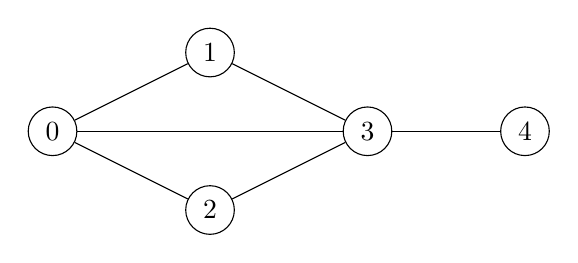
\begin{tikzpicture}
        \node[draw, circle] (0) at (0,1) {0};
        \node[draw, circle] (1) at (2,2) {1};
        \node[draw, circle] (2) at (2,0) {2};
        \node[draw, circle] (3) at (4,1) {3};
        \node[draw, circle] (4) at (6,1) {4};

        \draw (0) -- (1);
        \draw (0) -- (2);
        \draw (0) -- (3);
        \draw (1) -- (3);
        \draw (2) -- (3);
        \draw (3) -- (4);
    \end{tikzpicture}
\end{center}
De esta manera, podemos representar visualmente la situación, mostando las materias y los conflictos entre ellas.

\subsection{Modelo base}
El grafo anterior se representa con este modelo: \\
Notar que la matriz $assignedTo_2$ está vacía porque aún no tenemos materias asignadas. \\
(El grafo no tiene colores).
\begin{center}
    \begin{minipage}{0.1 \textwidth}
        \centering
        \textbf{$\bigtriangleup$} \\[4pt]
        \rowcolors{1}{}{blue!80!white}
        \begin{tabular}{>{\columncolor{blue!80!white}\color{white}\centering}m{1em}}
            0 \\
            1 \\
            2 \\
            3 \\
            4 \\
            5 \\
            6 \\
            7 \\
        \end{tabular}
    \end{minipage}
    \begin{minipage}{0.25 \textwidth}
        \centering
        \textbf{Constantes} \\[4pt]
        \begin{tabular}{@{}c@{\hskip 1em}>{\columncolor{blue!80!white}\color{white}}c@{}}
            L        & 0 \\
            AN       & 1 \\
            AA       & 2 \\
            MC       & 3 \\
            MA       & 4 \\
            Manana   & 5 \\
            Mediodia & 6 \\
            Tarde    & 7 \\
        \end{tabular}
    \end{minipage}
    \begin{minipage}{0.2 \textwidth}
        \centering
        \textbf{$subject_1$} \\[4pt]
        \begin{tabular}{@{}c@{\hskip 1em}>{\columncolor{blue!80!white}\color{white}}c@{}}
            0 & 1 \\
            1 & 1 \\
            2 & 1 \\
            3 & 1 \\
            4 & 1 \\
            5 & 0 \\
            6 & 0 \\
            7 & 0 \\
        \end{tabular}
    \end{minipage}
    \begin{minipage}{0.1 \textwidth}
        \centering
        \textbf{$timeSlot_1$} \\[4pt]
        \begin{tabular}{@{}c@{\hskip 1em}>{\columncolor{blue!80!white}\color{white}}c@{}}
            0 & 0 \\
            1 & 0 \\
            2 & 0 \\
            3 & 0 \\
            4 & 0 \\
            5 & 1 \\
            6 & 1 \\
            7 & 1 \\
        \end{tabular}
    \end{minipage}
    \begin{minipage}{0.2 \textwidth}
        \centering
        \textbf{Franjas} \\[4pt]
        \begin{tabular}{c >{\columncolor{blue!80!white}\color{white}}c}
            Mañana & 5 \\
        \end{tabular}\\[2pt]
        \begin{tabular}{c >{\columncolor{red!80!white}\color{white}}c}
            Mediodía & 6 \\
        \end{tabular}\\[2pt]
        \begin{tabular}{c >{\columncolor{green!60!black}\color{white}}c}
            Tarde & 7 \\
        \end{tabular}
    \end{minipage}
    \begin{minipage}{0.4 \textwidth}
        \centering
        \textbf{$inConflict_2$} \\[4pt]
        \begin{tabular}{c@{\hskip 1em}*{8}{>{\columncolor{black}\color{white}}c}} % Aplica solo a columnas de datos
            % Encabezado (no tiene formato blanco)
            \rowcolor{white}
            \multicolumn{1}{c}{}           &
            \multicolumn{1}{c}{\textbf{0}} &
            \multicolumn{1}{c}{\textbf{1}} &
            \multicolumn{1}{c}{\textbf{2}} &
            \multicolumn{1}{c}{\textbf{3}} &
            \multicolumn{1}{c}{\textbf{4}} &
            \multicolumn{1}{c}{\textbf{5}} &
            \multicolumn{1}{c}{\textbf{6}} &
            \multicolumn{1}{c}{\textbf{7}}                                 \\
            % Cuerpo (tiene fondo azul y texto blanco)
            0                              & 0 & 1 & 1 & 1 & 0 & 0 & 0 & 0 \\
            1                              & 1 & 0 & 0 & 1 & 0 & 0 & 0 & 0 \\
            2                              & 1 & 0 & 0 & 1 & 0 & 0 & 0 & 0 \\
            3                              & 1 & 1 & 1 & 0 & 1 & 0 & 0 & 0 \\
            4                              & 0 & 0 & 0 & 1 & 0 & 0 & 0 & 0 \\
            5                              & 0 & 0 & 0 & 0 & 0 & 0 & 0 & 0 \\
            6                              & 0 & 0 & 0 & 0 & 0 & 0 & 0 & 0 \\
            7                              & 0 & 0 & 0 & 0 & 0 & 0 & 0 & 0 \\
        \end{tabular}
    \end{minipage}
    \begin{minipage}{0.4 \textwidth}
        \centering
        \textbf{$assignedTo_2$} \\[4pt]
        \begin{tabular}{c@{\hskip 1em}*{8}{>{\columncolor{blue!80!white}\color{white}}c}} % Aplica solo a columnas de datos
            % Encabezado (no tiene formato blanco)
            \rowcolor{white}
            \multicolumn{1}{c}{}           &
            \multicolumn{1}{c}{\textbf{0}} &
            \multicolumn{1}{c}{\textbf{1}} &
            \multicolumn{1}{c}{\textbf{2}} &
            \multicolumn{1}{c}{\textbf{3}} &
            \multicolumn{1}{c}{\textbf{4}} &
            \multicolumn{1}{c}{\textbf{5}} &
            \multicolumn{1}{c}{\textbf{6}} &
            \multicolumn{1}{c}{\textbf{7}}                                 \\
            % Cuerpo (tiene fondo azul y texto blanco)
            0                              & 0 & 0 & 0 & 0 & 0 & 0 & 0 & 0 \\
            1                              & 0 & 0 & 0 & 0 & 0 & 0 & 0 & 0 \\
            2                              & 0 & 0 & 0 & 0 & 0 & 0 & 0 & 0 \\
            3                              & 0 & 0 & 0 & 0 & 0 & 0 & 0 & 0 \\
            4                              & 0 & 0 & 0 & 0 & 0 & 0 & 0 & 0 \\
            5                              & 0 & 0 & 0 & 0 & 0 & 0 & 0 & 0 \\
            6                              & 0 & 0 & 0 & 0 & 0 & 0 & 0 & 0 \\
            7                              & 0 & 0 & 0 & 0 & 0 & 0 & 0 & 0 \\
        \end{tabular}
    \end{minipage}

\end{center}

\newpage

\subsection{Reestricciones}
Debemos considerar ciertas reestricciones para poder construir modelos válidos.

\subsubsection{Irreflexividad (Conflictos)}
Si tenemos bucles (nodos autorreflexivos), será imposible colorear el grafo. Por lo tanto, los nodos (materias) no pueden estar en conflicto consigo mismas.
\begin{center}
    $(\forall s :: \neg inConflict_2(s, s))$
\end{center}

\subsubsection{Irreflexividad (Franjas horarias)}
Los franjas horarias no pueden estar asignadas a sí mismas ni a otras franjas horarias.
\begin{center}
    $(\forall c :: \neg assignedTo_2(c, c)) \land \neg(\exists c' :: assignedTo_2(c, c') \lor assignedTo_2(c, c')))$
\end{center}

\subsubsection{Los conflictos son sólo entre materias}
No tiene sentido dos franjas horarias estén en conflicto, tampoco que una materia esté en conflicto con una franja horaria y viceversa.
\begin{center}
    $(\forall s, t :: state_2(s,t) \Rightarrow subject_1(s) \land subject_1(t) )$
\end{center}



\subsubsection{La asignación es entre materias y franjas horarias}
No tendría sentido que se asigne una franja horaria a una franja horaria, ni tampoco asignar una materia a otra.
\begin{center}
    $(\forall s, c :: assignedTo_2(s, c) \Rightarrow subject_1(s) \land timeSlot_1(c))$
\end{center}

\subsubsection{Simetría de conflictos}
Si una materia s está en conflicto con una materia t, entonces t está en conflicto con s.
\begin{center}
    $(\forall s, t :: inConflict_2(s,t) \Leftrightarrow inConflict_2(t, s))$
\end{center}
\subsubsection{Los conflictos se dan sólo entre materias}

Como \texttt{state\_2(s, t)} puede representar tanto un conflicto como una asignación, distinguimos los conflictos como aquellos pares $(s, t)$ donde $s \ne t$ (ya que las asignaciones son del tipo $s = t$). Por lo tanto, restringimos esta propiedad sólo a las celdas donde $s \ne t$:

\begin{center}
    $(\forall s, t :: state_2(s, t) = 1 \land s \ne t \Rightarrow subject_1(s) \land subject_1(t))$
\end{center}

\subsubsection{Todas las materias tienen una única franja horaria}
No queremos que se pueda asignar la misma materia a dos franjas horarias diferentes. En coloreo de grafos, es el equivalente a decir: "Los nodos sólo pueden estar pintados de un solo color".
\begin{center}
    $(\forall s :: subject_1(s) \Rightarrow (\exists c :: assignedTo_2(s, c) \land \
        (\forall x, x' :: (assignedTo_2(s, x) \land assignedTo_2(s, x')) \Rightarrow x = x' )
        ))$
\end{center}

\subsubsection{No hay materias en conflicto en la misma franja horaria}
Supongamos en caso en que dos materias están en conflicto porque comparten estudiantes, si se ponen en la misma franja horaria, los estudiantes no podrán asistir a las dos clases al mismo tiempo.
\begin{center}
    $\neg(\exists s, t, c :: inConflict_2(s, t) \land assignedTo_2(s, c) \land assignedTo_2(t, c) )$
\end{center}

\subsubsection{Las materias no son franjas horarias y las franjas horarias no son materias}
\begin{center}
    $(\forall x :: subject_1(x) \lor timeSlot_1(x)) \land \neg(\exists x :: subject_1(x) \land timeSlot_1(x))$
\end{center}

\subsubsection{Hay exactamente 3 franjas horarias}
\begin{center}
    \(
    timeSlot_1(Manana) \land timeSlot_1(Mediodia) \land timeSlot_1(Tarde) \\
    \land\ (Manana \not= Mediodia) \land (Mediodia \not= Tarde) \land (Manana \not= Tarde) \\
    \land\ (\forall x :: timeSlot_1(x) \Rightarrow (x = Manana \lor x = Mediodia \lor x = Tarde))
    \)
\end{center}

\subsubsection{Hay exactamente 5 materias}
\begin{center}
    \(
    subject_1(L) \land subject_1(AN) \land subject_1(AA) \land subject_1(MC) \land subject_1(MA) \\
    \land\ (L \not= AN) \land (L \not= AA) \land (L \not= MC) \land (L \not= MA) \\
    \land\ (AN \not= AA) \land (AN \not= MC) \land (AN \not= MA) \\
    \land\ (AA \not= MC) \land (AA \not= MA) \land (MC \not= MA) \\
    \land\ (\forall x :: subject_1(x) \Rightarrow (x = L \lor x = AN \lor x = AA \lor x = MC \lor x = MA))
    \)
\end{center}

\subsubsection{Los conflictos de mi problema son:}
\[
    \begin{aligned}
                & inConflict_2(L, AN) \land inConflict_2(AN, L)   \\
        \land\  & inConflict_2(L, AA) \land inConflict_2(AA, L)   \\
        \land\  & inConflict_2(L, MC) \land inConflict_2(MC, L)   \\
        \land\  & inConflict_2(L, MA) \land inConflict_2(MA, L)   \\
        \land\  & inConflict_2(AN, AA) \land inConflict_2(AA, AN) \\
        \land\  & inConflict_2(AN, MC) \land inConflict_2(MC, AN) \\
        \land\  & inConflict_2(AN, MA) \land inConflict_2(MA, AN) \\
        \land\  & inConflict_2(AA, MC) \land inConflict_2(MC, AA) \\
        \land\  & inConflict_2(AA, MA) \land inConflict_2(MA, AA) \\
        \land\  & inConflict_2(MC, MA) \land inConflict_2(MA, MC)
    \end{aligned}
\]

\newpage

\subsection{Modelo que plantea una solución}
\begin{center}
    \begin{minipage}{0.1 \textwidth}
        \centering
        \textbf{$\bigtriangleup$} \\[4pt]
        \rowcolors{1}{}{blue!80!white}
        \begin{tabular}{>{\columncolor{blue!80!white}\color{white}\centering}m{1em}}
            0 \\
            1 \\
            2 \\
            3 \\
            4 \\
            5 \\
            6 \\
            7 \\
        \end{tabular}
    \end{minipage}
    \begin{minipage}{0.25 \textwidth}
        \centering
        \textbf{Constantes} \\[4pt]
        \begin{tabular}{@{}c@{\hskip 1em}>{\columncolor{blue!80!white}\color{white}}c@{}}
            L        & 0 \\
            AN       & 1 \\
            AA       & 2 \\
            MC       & 3 \\
            MA       & 4 \\
            Manana   & 5 \\
            Mediodia & 6 \\
            Tarde    & 7 \\
        \end{tabular}
    \end{minipage}
    \begin{minipage}{0.2 \textwidth}
        \centering
        \textbf{$subject_1$} \\[4pt]
        \begin{tabular}{@{}c@{\hskip 1em}>{\columncolor{blue!80!white}\color{white}}c@{}}
            0 & 1 \\
            1 & 1 \\
            2 & 1 \\
            3 & 1 \\
            4 & 1 \\
            5 & 0 \\
            6 & 0 \\
            7 & 0 \\
        \end{tabular}
    \end{minipage}
    \begin{minipage}{0.1 \textwidth}
        \centering
        \textbf{$timeSlot_1$} \\[4pt]
        \begin{tabular}{@{}c@{\hskip 1em}>{\columncolor{blue!80!white}\color{white}}c@{}}
            0 & 0 \\
            1 & 0 \\
            2 & 0 \\
            3 & 0 \\
            4 & 0 \\
            5 & 1 \\
            6 & 1 \\
            7 & 1 \\
        \end{tabular}
    \end{minipage}
    \begin{minipage}{0.2 \textwidth}
        \centering
        \textbf{Franjas} \\[4pt]
        \begin{tabular}{c >{\columncolor{blue!80!white}\color{white}}c}
            Mañana & 5 \\
        \end{tabular}\\[2pt]
        \begin{tabular}{c >{\columncolor{red!80!white}\color{white}}c}
            Mediodía & 6 \\
        \end{tabular}\\[2pt]
        \begin{tabular}{c >{\columncolor{green!60!black}\color{white}}c}
            Tarde & 7 \\
        \end{tabular}
    \end{minipage}
    \begin{minipage}{0.4 \textwidth}
        \centering
        \textbf{$inConflict_2$} \\[4pt]
        \begin{tabular}{c@{\hskip 1em}*{8}{>{\columncolor{black}\color{white}}c}} % Aplica solo a columnas de datos
            % Encabezado (no tiene formato blanco)
            \rowcolor{white}
            \multicolumn{1}{c}{}           &
            \multicolumn{1}{c}{\textbf{0}} &
            \multicolumn{1}{c}{\textbf{1}} &
            \multicolumn{1}{c}{\textbf{2}} &
            \multicolumn{1}{c}{\textbf{3}} &
            \multicolumn{1}{c}{\textbf{4}} &
            \multicolumn{1}{c}{\textbf{5}} &
            \multicolumn{1}{c}{\textbf{6}} &
            \multicolumn{1}{c}{\textbf{7}}                                 \\
            % Cuerpo (tiene fondo azul y texto blanco)
            0                              & 0 & 1 & 1 & 1 & 0 & 0 & 0 & 0 \\
            1                              & 1 & 0 & 0 & 1 & 0 & 0 & 0 & 0 \\
            2                              & 1 & 0 & 0 & 1 & 0 & 0 & 0 & 0 \\
            3                              & 1 & 1 & 1 & 0 & 1 & 0 & 0 & 0 \\
            4                              & 0 & 0 & 0 & 1 & 0 & 0 & 0 & 0 \\
            5                              & 0 & 0 & 0 & 0 & 0 & 0 & 0 & 0 \\
            6                              & 0 & 0 & 0 & 0 & 0 & 0 & 0 & 0 \\
            7                              & 0 & 0 & 0 & 0 & 0 & 0 & 0 & 0 \\
        \end{tabular}
    \end{minipage}
    \begin{minipage}{0.4 \textwidth}
        \centering
        \textbf{$assignedTo_2$} \\[4pt]
        \begin{tabular}{c@{\hskip 1em}*{8}{>{\columncolor{blue!80!white}\color{white}}c}} % Aplica solo a columnas de datos
            % Encabezado (no tiene formato blanco)
            \rowcolor{white}
            \multicolumn{1}{c}{}           &
            \multicolumn{1}{c}{\textbf{0}} &
            \multicolumn{1}{c}{\textbf{1}} &
            \multicolumn{1}{c}{\textbf{2}} &
            \multicolumn{1}{c}{\textbf{3}} &
            \multicolumn{1}{c}{\textbf{4}} &
            \multicolumn{1}{c}{\textbf{5}} &
            \multicolumn{1}{c}{\textbf{6}} &
            \multicolumn{1}{c}{\textbf{7}}                                 \\
            % Cuerpo (tiene fondo azul y texto blanco)
            0                              & 0 & 0 & 0 & 0 & 0 & 0 & 0 & 1 \\
            1                              & 0 & 0 & 0 & 0 & 0 & 1 & 0 & 0 \\
            2                              & 0 & 0 & 0 & 0 & 0 & 1 & 0 & 0 \\
            3                              & 0 & 0 & 0 & 0 & 0 & 0 & 1 & 0 \\
            4                              & 0 & 0 & 0 & 0 & 0 & 1 & 0 & 0 \\
            5                              & 0 & 0 & 0 & 0 & 0 & 0 & 0 & 0 \\
            6                              & 0 & 0 & 0 & 0 & 0 & 0 & 0 & 0 \\
            7                              & 0 & 0 & 0 & 0 & 0 & 0 & 0 & 0 \\
        \end{tabular}
    \end{minipage}
\end{center}
\begin{center}
    \textbf{$state_2$ (fusionado)} \\[4pt]
    \begin{tabular}{c@{\hskip 1em}*{8}{c}}
        \rowcolor{white}
          & \textbf{0}             & \textbf{1}             & \textbf{2}             & \textbf{3}             & \textbf{4}             & \textbf{5}           & \textbf{6}           & \textbf{7}           \\
        0 & \cellcolor{white}0     & \cellcolor{yellow!40}1 & \cellcolor{yellow!40}1 & \cellcolor{yellow!40}1 & \cellcolor{white}0     & \cellcolor{white}0   & \cellcolor{white}0   & \cellcolor{gray!30}1 \\
        1 & \cellcolor{yellow!40}1 & \cellcolor{white}0     & \cellcolor{white}0     & \cellcolor{yellow!40}1 & \cellcolor{white}0     & \cellcolor{gray!30}1 & \cellcolor{white}0   & \cellcolor{white}0   \\
        2 & \cellcolor{yellow!40}1 & \cellcolor{white}0     & \cellcolor{white}0     & \cellcolor{yellow!40}1 & \cellcolor{white}0     & \cellcolor{gray!30}1 & \cellcolor{white}0   & \cellcolor{white}0   \\
        3 & \cellcolor{yellow!40}1 & \cellcolor{yellow!40}1 & \cellcolor{yellow!40}1 & \cellcolor{white}0     & \cellcolor{yellow!40}1 & \cellcolor{white}0   & \cellcolor{gray!30}1 & \cellcolor{white}0   \\
        4 & \cellcolor{white}0     & \cellcolor{white}0     & \cellcolor{white}0     & \cellcolor{yellow!40}1 & \cellcolor{white}0     & \cellcolor{gray!30}1 & \cellcolor{white}0   & \cellcolor{white}0   \\
        5 & \cellcolor{white}0     & \cellcolor{white}0     & \cellcolor{white}0     & \cellcolor{white}0     & \cellcolor{white}0     & \cellcolor{white}0   & \cellcolor{white}0   & \cellcolor{white}0   \\
        6 & \cellcolor{white}0     & \cellcolor{white}0     & \cellcolor{white}0     & \cellcolor{white}0     & \cellcolor{white}0     & \cellcolor{white}0   & \cellcolor{white}0   & \cellcolor{white}0   \\
        7 & \cellcolor{white}0     & \cellcolor{white}0     & \cellcolor{white}0     & \cellcolor{white}0     & \cellcolor{white}0     & \cellcolor{white}0   & \cellcolor{white}0   & \cellcolor{white}0   \\
    \end{tabular}

    \vspace{1em}
    \textbf{Leyenda:}

    \begin{tabular}{ll}
        \cellcolor{white}0     & Vacío                         \\
        \cellcolor{yellow!40}1 & En conflicto (`inConflict_2`) \\
        \cellcolor{gray!30}1   & Asignado (`assignedTo_2`)     \\
    \end{tabular}
\end{center}
\begin{center}
    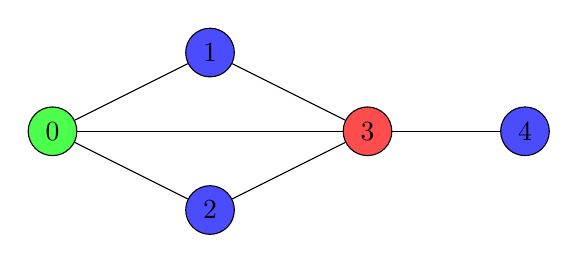
\begin{tikzpicture}
        \node[draw, circle, fill=green!70] (0) at (0,1) {0};
        \node[draw, circle, fill=blue!70] (1) at (2,2) {1};
        \node[draw, circle, fill=blue!70] (2) at (2,0) {2};
        \node[draw, circle, fill=red!70] (3) at (4,1) {3};
        \node[draw, circle, fill=blue!70] (4) at (6,1) {4};

        \draw (0) -- (1);
        \draw (0) -- (2);
        \draw (0) -- (3);
        \draw (1) -- (3);
        \draw (2) -- (3);
        \draw (3) -- (4);
    \end{tikzpicture}
\end{center}

Este modelo presenta una solución al problema asignando:
\begin{itemize}
    \item Mañana (Azul): Algoritmos Naza, Algoritmos Ariel, Matemática para Agronomía.
    \item Mediodia (Rojo): Matemática para Computación.
    \item Tarde (Verde): Lógica.
\end{itemize}

\subsection{Satisfacibilidad del modelo solución propuesto}














\newpage

\section{Asignación de materias a franjas horarias (Usando una sola matriz)}

Se presenta la siguiente situación problemática:

En la universidad, cursamos cinco materias: \textbf{Lógica}, \textbf{Algoritmos (Naza)}, \textbf{Algoritmos (Ariel)}, \textbf{Matemática para Computación} y \textbf{Matemática para Agronomía}. Disponemos de tres franjas horarias posibles: \textbf{Mañana}, \textbf{Mediodía} y \textbf{Tarde}. El objetivo es asignar cada materia a una franja horaria, de forma tal que no se produzcan conflictos.

Modelaremos esta situación como un \textbf{problema de coloreo de grafos}, lo cual nos permitirá aplicar técnicas formales para encontrar una solución válida.

\begin{itemize}
    \item Cada \textbf{materia} será representada por un \textbf{nodo}.
    \item Cada \textbf{franja horaria} será representada por un \textbf{color}.
    \item Cada \textbf{conflicto} entre materias será representado por una \textbf{arista} entre nodos.
\end{itemize}

Definimos que existe un \textbf{conflicto} entre dos materias si:
\begin{itemize}
    \item Comparten estudiantes, o
    \item Son dictadas por el mismo docente.
\end{itemize}

Por ejemplo, si \textbf{Lógica} y \textbf{Matemática para Computación} son dictadas por el mismo profesor, entonces hay un conflicto entre ambas, por lo que deben asignarse a franjas horarias distintas.

La estructura concreta de los conflictos es la siguiente:
\begin{itemize}
    \item \textbf{Lógica} está en conflicto con \textbf{Algoritmos (Naza)} (comparten alumnos).
    \item \textbf{Lógica} está en conflicto con \textbf{Algoritmos (Ariel)} (comparten alumnos).
    \item \textbf{Lógica} está en conflicto con \textbf{Matemática para Computación} (comparten alumnos).
    \item \textbf{Algoritmos (Naza)} está en conflicto con \textbf{Matemática para Computación} (comparten alumnos).
    \item \textbf{Algoritmos (Ariel)} está en conflicto con \textbf{Matemática para Computación} (comparten alumnos).
    \item \textbf{Matemática para Computación} está en conflicto con \textbf{Matemática para Agronomía} (comparten docente).
\end{itemize}

\newpage

\subsection{Grafo sin colorear}

Para representar esta situación, usamos un grafo sin colorear, donde los nodos corresponden a las materias de la siguiente manera:

\begin{itemize}
    \item 0: Lógica
    \item 1: Algoritmos (Naza)
    \item 2: Algoritmos (Ariel)
    \item 3: Matemática para Computación
    \item 4: Matemática para Agronomía
\end{itemize}

\begin{center}
    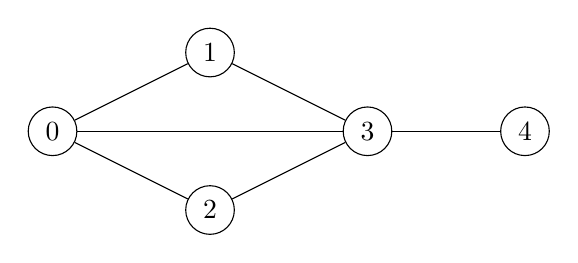
\begin{tikzpicture}
        \node[draw, circle] (0) at (0,1) {0};
        \node[draw, circle] (1) at (2,2) {1};
        \node[draw, circle] (2) at (2,0) {2};
        \node[draw, circle] (3) at (4,1) {3};
        \node[draw, circle] (4) at (6,1) {4};

        \draw (0) -- (1);
        \draw (0) -- (2);
        \draw (0) -- (3);
        \draw (1) -- (3);
        \draw (2) -- (3);
        \draw (3) -- (4);
    \end{tikzpicture}
\end{center}
De esta manera, podemos representar visualmente la situación, mostando las materias y los conflictos entre ellas.

\subsection{Modelo base}
El grafo anterior se representa con este modelo: \\
Notar que la matriz $assignedTo_2$ está vacía porque aún no tenemos materias asignadas. \\
(El grafo no tiene colores).
\begin{center}
    \begin{minipage}{0.1 \textwidth}
        \centering
        \textbf{$\bigtriangleup$} \\[4pt]
        \rowcolors{1}{}{blue!80!white}
        \begin{tabular}{>{\columncolor{blue!80!white}\color{white}\centering}m{1em}}
            0 \\
            1 \\
            2 \\
            3 \\
            4 \\
            5 \\
            6 \\
            7 \\
        \end{tabular}
    \end{minipage}
    \begin{minipage}{0.25 \textwidth}
        \centering
        \textbf{Constantes} \\[4pt]
        \begin{tabular}{@{}c@{\hskip 1em}>{\columncolor{blue!80!white}\color{white}}c@{}}
            L        & 0 \\
            AN       & 1 \\
            AA       & 2 \\
            MC       & 3 \\
            MA       & 4 \\
            Manana   & 5 \\
            Mediodia & 6 \\
            Tarde    & 7 \\
        \end{tabular}
    \end{minipage}
    \begin{minipage}{0.2 \textwidth}
        \centering
        \textbf{$subject_1$} \\[4pt]
        \begin{tabular}{@{}c@{\hskip 1em}>{\columncolor{blue!80!white}\color{white}}c@{}}
            0 & 1 \\
            1 & 1 \\
            2 & 1 \\
            3 & 1 \\
            4 & 1 \\
            5 & 0 \\
            6 & 0 \\
            7 & 0 \\
        \end{tabular}
    \end{minipage}
    \begin{minipage}{0.1 \textwidth}
        \centering
        \textbf{$timeSlot_1$} \\[4pt]
        \begin{tabular}{@{}c@{\hskip 1em}>{\columncolor{blue!80!white}\color{white}}c@{}}
            0 & 0 \\
            1 & 0 \\
            2 & 0 \\
            3 & 0 \\
            4 & 0 \\
            5 & 1 \\
            6 & 1 \\
            7 & 1 \\
        \end{tabular}
    \end{minipage}
    \begin{minipage}{0.2 \textwidth}
        \centering
        \textbf{Franjas} \\[4pt]
        \begin{tabular}{c >{\columncolor{blue!80!white}\color{white}}c}
            Mañana & 5 \\
        \end{tabular}\\[2pt]
        \begin{tabular}{c >{\columncolor{red!80!white}\color{white}}c}
            Mediodía & 6 \\
        \end{tabular}\\[2pt]
        \begin{tabular}{c >{\columncolor{green!60!black}\color{white}}c}
            Tarde & 7 \\
        \end{tabular}
    \end{minipage}
    \vspace{1em}
    \begin{minipage}{0.5\textwidth}
        \textbf{$state_2$} \\[4pt]
        \begin{tabular}{c|c|c|c|c|c|c|c|c|}
              & \textbf{0} & \textbf{1} & \textbf{2} & \textbf{3} & \textbf{4} & \textbf{5} & \textbf{6} & \textbf{7} \\
            \hline
            0 & \void      & \conf      & \conf      & \conf      & \void      & \void      & \void      & \void      \\
            \hline
            1 & \conf      & \void      & \void      & \conf      & \void      & \void      & \void      & \void      \\
            \hline
            2 & \conf      & \void      & \void      & \conf      & \void      & \void      & \void      & \void      \\
            \hline
            3 & \conf      & \conf      & \conf      & \void      & \conf      & \void      & \void      & \void      \\
            \hline
            4 & \void      & \void      & \void      & \conf      & \void      & \void      & \void      & \void      \\
            \hline
            5 & \void      & \void      & \void      & \void      & \void      & \void      & \void      & \void      \\
            \hline
            6 & \void      & \void      & \void      & \void      & \void      & \void      & \void      & \void      \\
            \hline
            7 & \void      & \void      & \void      & \void      & \void      & \void      & \void      & \void      \\
            \hline
        \end{tabular}
    \end{minipage}
    \begin{minipage}{0.4 \textwidth}
        \textbf{Leyenda:}
        \begin{tabular}{ll}
            \cellcolor{white}0     & Vacío                           \\
            \cellcolor{yellow!40}1 & En conflicto (`$inConflict_2$`) \\
            \cellcolor{gray!30}1   & Asignado (`$assignedTo_2$`)     \\
        \end{tabular}
    \end{minipage}

\end{center}

\newpage

\subsection{Reestricciones}
Debemos considerar ciertas reestricciones para poder construir modelos válidos.


\subsubsection{Irreflexividad ($\varphi_1$):}
\begin{center}
    $(\forall s :: \neg \, state_2(s, s))$
\end{center}
Ninguna materia está en conflicto consigo misma. Ni Ninguna franja se asigna a sí misma.
\subsubsection{No hay conflictos o asignacion entre dos franjas distintas ($\varphi_2$)}
\begin{center}
    $\neg(\exists s, t \,::\, timeSlot_1(s) \land timeSlot_1(t) \land s \neq t \land state_2(s, t))$ \\
\end{center}
No hay conflicto ni asignación de una franja a otra franja diferente (no hay conflicto o asignación franja–franja)

\subsubsection{Conflictos solo entre materias ($\varphi_3$):}
\begin{center}
    $(\forall s, t \,::\, subject_1(t) \land state_2(s,t) \rightarrow subject_1(s))$
\end{center}
Si $state_2(s,t)$ representa un conflicto (y $t$ es una materia), entonces $s$ también debe ser una materia.

\subsubsection{Asignación entre materia y franja ($\varphi_4$):}
\begin{center}
    $(\forall s, t \,::\, timeSlot_1(t) \land state_2(s,t) \rightarrow subject_1(s))$
\end{center}
Si $state_2(s,t)$ representa una asignación (y $t$ es una franja horaria), entonces $s$ debe ser una materia.

\item \textbf{Simetría de conflictos ($\varphi_5$):}
\begin{center}
    $(\forall s, t \,::\, subject_1(s) \land subject_1(t) \land state_2(s, t) \rightarrow state_2(t, s))$
\end{center}
El conflicto es bidireccional: si $s$ y $t$ son materias y $s$ está en conflicto con $t$, entonces $t$ debería estar en conflicto con $s$.

\item \textbf{Única franja por materia ($\varphi_6$):}
\begin{center}
    $\forall s \, (0 \leq s \leq 4 \rightarrow \exists ! t \, (5 \leq t \leq 7 \land state_2(s,t)))$
\end{center}
Cada materia $s \in \{0, \dots, 4\}$ tiene exactamente una franja $t \in \{5, 6, 7\}$ asignada.

\item \textbf{No hay materias en conflicto en la misma franja ($\varphi_7$):}
\begin{center}
    $\forall x,y \, ((0 \leq x \leq 4 \land 0 \leq y \leq 4 \land state_2(x,y)) \rightarrow \forall r \, (5 \leq r \leq 7 \rightarrow \neg (state_2(x,r) \land state_2(y,r))))$
\end{center}
Si $x$ y $y$ son materias en conflicto ($state_2(x,y)$), no pueden compartir la misma franja $r$.

\item \textbf{Materias y franjas disjuntas ($\varphi_8$):}
\begin{center}
    $\forall x \, (0 \leq x \leq 4 \rightarrow \neg (5 \leq x \leq 7))$
\end{center}
Ningún número corresponde simultáneamente a materia y a franja. (Los índices $0 \dots 4$ son materias, $5 \dots 7$ son franjas).

\item \textbf{Exactamente 3 franjas horarias ($\varphi_9$):}
\begin{center}
    $\forall t \, ((5 \leq t \leq 7) \leftrightarrow (t = 5 \lor t = 6 \lor t = 7))$
\end{center}
Solo existen tres valores para franjas: 5, 6 y 7.

\item \textbf{Exactamente 5 materias ($\varphi_{10}$):}
\begin{center}
    $\forall s \, ((0 \leq s \leq 4) \leftrightarrow (s = 0 \lor s = 1 \lor s = 2 \lor s = 3 \lor s = 4))$
\end{center}
Solo existen cinco valores para materias: 0, 1, 2, 3 y 4.

\item \textbf{Conflictos explícitos del problema ($\varphi_{11}$):}
\begin{center}
    $state_2(0,1) \land state_2(0,4) \land state_2(1,2) \land state_2(2,3)$
\end{center}
(Ejemplo de conflictos dados en el problema: materia 0 con 1, 0 con 4, 1 con 2, y 2 con 3. Por simetría también valdrían los inversos.)

\end{document}
